\chapter{Introduction}

\section{Overview}

The ForSyDe model of the ASK uses the following computational models.

\begin{itemize}
\item Untimed model (SDF)
\item Synchronous model (SR)
\item Continuous time model (CT) 
\end{itemize}

The example can be downloaded from the ANDRES homepage. In order to run the model we need a version of the ForSyDe standard library that includes the new library for continuous time models. Since the CT-library is still under development, there is no stable release with it available. However, an intermediate version can be downloaded from the ANDRES homepage. 

The structure of the ForSyDe model is shown in Figure \ref{fig:Overview}.

\begin{figure}[htb!]
\centering%
\resizebox{\columnwidth}{!}{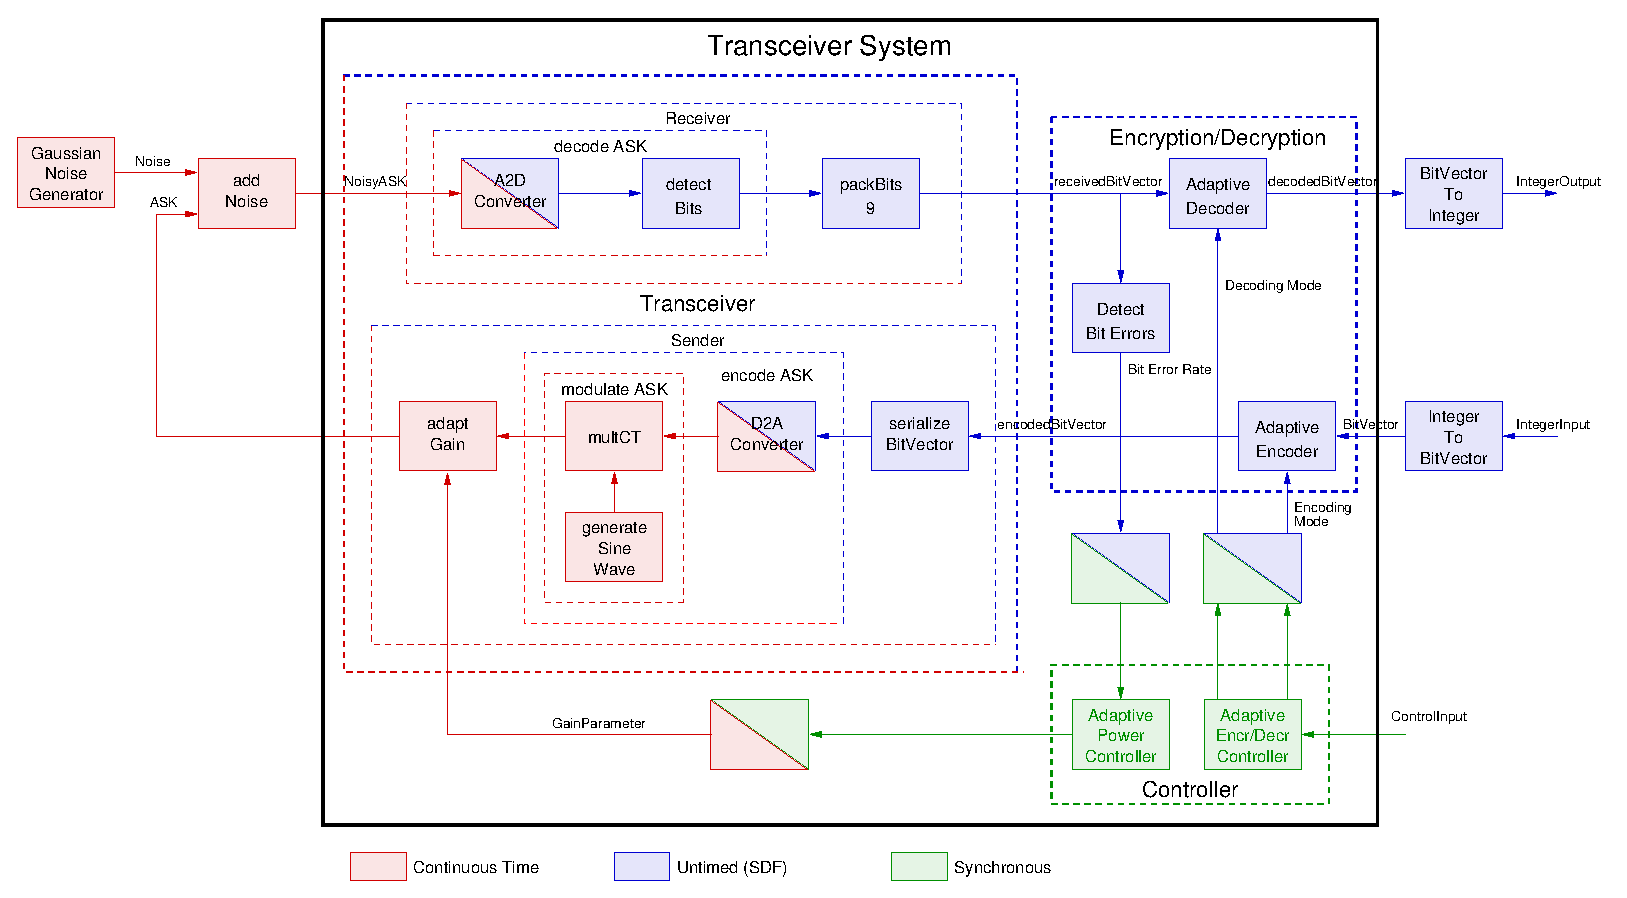
\includegraphics{fig/TestBench.eps}}
\caption{The Structure of ASK transceiver case study}
\label{fig:Overview}
\end{figure}

All signal names shown in the figure can be accessed, if the ForSyDe model is executed with a Haskell interpreter like \texttt{hugs}\footnote{\texttt{hugs} can be downloaded from \url{http://haskell.org/hugs}} or \texttt{ghci}\footnote{\texttt{ghci} is part of the Glasgow Haskell Compiler, which can be downloaded from \url{http://haskell.org/ghc/}}. 


\subsection{Installation}
\label{sec:Installation}

We assume in the following that you are using a UNIX environment.

\begin{enumerate} 
\item Make a directory \texttt{ForSyDeExample} somewhere in your directory structure. Enter this directory.
\item Download the file \texttt{ForSyDeStdLib.zip} from the ANDRES homepage
\item Download the file \texttt{ToyExample.zip} from the ANDRES homepage
\item Extract the ForSyDe library so that it is located under the directory \texttt{ForSyDeExample}
\item Extract the toy example so that it is located under the directory \texttt{ForSyDeExample}
\item Create an environment variable \texttt{\$FORSYDELIB} that points to the directory \texttt{ForSyDeStdLib}
\item Move to the directory for the toy example
\item Start your Haskell interpreter with
  \begin{itemize}
  \item \texttt{hugs -P:\$FORSYDELIB} (for \texttt{hugs})
  \item \texttt{>ghci -i\$FORSYDELIB} (for \texttt{ghci})
\end{itemize}
\item Then load the testbench, which includes all the modules with \texttt{:l TestBench}. 
\item Then start the simulation by \texttt{main}.
\item You should now see something like this.
\begin{verbatim}
>hugs -P:\$FORSYDELIB
__   __ __  __  ____   ___      _________________________________________
||   || ||  || ||  || ||__      Hugs 98: Based on the Haskell 98 standard
||___|| ||__|| ||__||  __||     Copyright (c) 1994-2005
||---||         ___||           World Wide Web: http://haskell.org/hugs
||   ||                         Report bugs to: hugs-bugs@haskell.org
||   || Version: May 2006       _________________________________________

Haskell 98 mode: Restart with command line option -98 to enable extensions

Type :? for help
Hugs> :l Main
Main> main
Testing ...
Input signal of integers
input = {0,1,2,3,4}
Output signal of integers
output = {0,40,2,3,4}
Signal plotted.
Signal plotted.
Signal plotted.
Done!
\end{verbatim}

\item Three plots are generated during the execution of the model.

\begin{figure}[htb!]
\centering%
\resizebox{\columnwidth}{!}{\includegraphics{fig/ct-moc-graph-sig_ct_waveSent.eps}}
\caption{The signal \texttt{sig\_ct\_waveSent}}
\label{fig:ASK}
\end{figure}

\begin{figure}[htb!]
\centering%
\resizebox{\columnwidth}{!}{\includegraphics{fig/ct-moc-graph-sig_ct_waveReceived.eps}}
\caption{The signal \texttt{sig\_ct\_waveReceived}}
\label{fig:NoisyASK}
\end{figure}

\begin{figure}[htb!]
\centering%
\resizebox{\columnwidth}{!}{\includegraphics{fig/ct-moc-graph-sig_ct_lpout.eps}}
\caption{The signal \texttt{sig\_ct\_lpout}}
\label{fig:FilteredNoisyASK}
\end{figure}
As can be seen in the figures, the gain is increased to a higher level after an increase of the bit error rate. The 2nd input signal '1' was received as a '40'. 
\item You can also look at exported internal signals like the interfaces between the subsystems of Figure \ref{fig:Overview}.
\begin{verbatim}
Main> bitErrorRate
{0,1,0,0,0}
\end{verbatim}
\end{enumerate}



%%% Local Variables: 
%%% mode: latex
%%% TeX-master: "ASK"
%%% End: 
